\documentclass[lang=ngerman]{edoxarticle}

\renewcommand\examname{Klausur 1}

\begin{document}
\pdate{}
\begin{exam}{Mathematik EF GK}

\wssection[A]{Prüfungsteil A: Aufgaben ohne Hilfsmittel}
\vskip10pt
\textbf{Hinweis:} Für Prüfungsteil A sind außer Zeichengeräten keine Hilfsmittel zugelassen.
\vskip10pt
\exercise*[Aufgabe 1]{
\subexercise{
Betrachten Sie die Zuordnung zwischen den Schülerinnen und Schülern einer Klasse und ihren Geburtsdaten.

(i) Ist die Zuordnung \emph{Schüler $\to$ Geburtsdatum} eine Funktion? Begründen Sie.

(ii) Ist die Zuordnung \emph{Geburtsdatum $\to$ Schüler} eine Funktion? Begründen Sie.
\solve{
(i) Es liegt eine Funktion vor, da jeder Schüler genau ein Geburtsdatum besitzt.\pp[2]

(ii) Es liegt \textbf{keine} Funktion vor: Haben zwei Schüler am selben Tag Geburtstag, wird diesem Geburtsdatum mehr als ein Schüler zugeordnet -- die Zuordnung ist dann nicht eindeutig.\pp
}
}

\subexercise{
Entscheiden Sie allein anhand der Exponenten, ob der Graph von
\[
f(x)=3x^4-x^2+5
\]
achsensymmetrisch zur $y$-Achse, punktsymmetrisch zum Ursprung oder keins von beidem ist.
\solve{
Nur gerade Exponenten $\Rightarrow$ achsensymmetrisch zur $y$-Achse.\pp
}
}

\subexercise{
Weisen Sie rechnerisch nach, ob der Graph von
\[
g(x)=-x^5+2x^3-x
\]
achsensymmetrisch zur $y$-Achse oder punktsymmetrisch zum Ursprung ist.
\solve{
\[
g(-x)=-(-x)^5+2(-x)^3-(-x)=x^5-2x^3+x=-\left(-x^5+2x^3-x\right)=-g(x)
\]
Also ist der Graph punktsymmetrisch zum Ursprung.\pp[2]
}
}

\subexercise{
Gegeben ist die Funktion $f$ mit
\[
f(x)=-x^3+4x.
\]
Eine der drei Abbildungen zeigt den Graphen von $f$. Geben Sie die passende Abbildung an und begründen Sie Ihre Entscheidung mithilfe von Symmetrie und Randverhalten.

\begin{center}
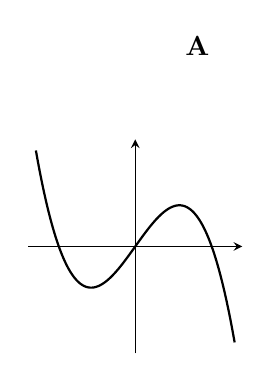
\begin{tikzpicture}
\begin{axis}[width=4.3cm,height=4.3cm,axis lines=middle,xmin=-2.8,xmax=2.8,ymin=-8,ymax=8,xtick=\empty,ytick=\empty,samples=100,domain=-2.6:2.6]
\addplot[thick] {-x^3+4*x};
\end{axis}
\node at (2.15,3.9) {\textbf{A}};
\end{tikzpicture}
\hfill
\begin{tikzpicture}
\begin{axis}[width=4.3cm,height=4.3cm,axis lines=middle,xmin=-2.8,xmax=2.8,ymin=-8,ymax=8,xtick=\empty,ytick=\empty,samples=100,domain=-2.6:2.6]
\addplot[thick] {-0.3*x^4+2*x^2};
\end{axis}
\node at (2.15,3.9) {\textbf{B}};
\end{tikzpicture}
\hfill
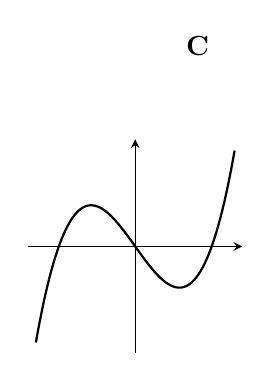
\begin{tikzpicture}
\begin{axis}[width=4.3cm,height=4.3cm,axis lines=middle,xmin=-2.8,xmax=2.8,ymin=-8,ymax=8,xtick=\empty,ytick=\empty,samples=100,domain=-2.6:2.6]
\addplot[thick] {x^3-4*x};
\end{axis}
\node at (2.15,3.9) {\textbf{C}};
\end{tikzpicture}
\end{center}
\solve{
$f$ enthält nur ungerade Exponenten, ist also punktsymmetrisch zum Ursprung -- das schließt Abbildung B (achsensymmetrisch) aus.

Der führende Term von $f$ ist $-x^3$, also negatives Vorzeichen bei ungeradem Grad $3$: für $x\to\infty$ gilt $f(x)\to-\infty$, für $x\to-\infty$ gilt $f(x)\to\infty$. In Abbildung C verhält es sich umgekehrt (führender Term $+x^3$).

Damit passt \textbf{Abbildung A}.\pp
}
}
}

\newpage
\exercise*[Aufgabe 2]{
Gegeben sind die Funktionen
\[
f(x)=-2x^5+3x^2-1 \qquad\text{und}\qquad g(x)=0{,}5x^4-6x+2.
\]
\subexercise{
Geben Sie den Grad von $f$ und $g$ an.
\solve{
$f$ hat Grad $5$, $g$ hat Grad $4$.\pp
}
}
\vskip8pt
\subexercise{
Beschreiben Sie das Verhalten von $f$ und $g$ für $x\to\infty$ sowie $x\to-\infty$.
\solve{
Der führende Term von $f$ ist $-2x^5$ (ungerader Grad, negatives Vorzeichen): $f(x)\to-\infty$ für $x\to\infty$ und $f(x)\to\infty$ für $x\to-\infty$.\pp

Der führende Term von $g$ ist $0{,}5x^4$ (gerader Grad, positives Vorzeichen): $g(x)\to\infty$ für $x\to\infty$ und für $x\to-\infty$.\pp
}
}
\vskip8pt
\subexercise{
Bestimmen Sie die Nullstellen durch Ausklammern.
\[
f(x)=x^3-9x
\]
\solve{
\[
x^3-9x=x(x^2-9)=x(x-3)(x+3)
\]
\[
x_1=0,\quad x_2=3,\quad x_3=-3
\]
\pp[2]
}
}
\vskip8pt
\subexercise{
Gegeben ist die Funktion $h(x)=x^4+2x^2+1$. Geben Sie an, wie viele Nullstellen $h$ höchstens besitzen kann.
\solve{
Grad $4$ $\Rightarrow$ höchstens $4$ Nullstellen.\pp
}
}
}

\newpage
\wssection[B]{Prüfungsteil B: Aufgaben mit Hilfsmitteln}
\vskip10pt
\exercise*[Aufgabe 3]{
Die Körpertemperatur eines Patienten wird über einen Zeitraum von $24$ Stunden beobachtet. Sie steigt zunächst von $37\,^\circ\mathrm C$ auf einen Höchstwert von etwa $39{,}7\,^\circ\mathrm C$ an und fällt danach langsam wieder ab. Der Verlauf wird für $0\le t\le24$ modelliert durch
\[
f(t)=0{,}00074t^3-0{,}04667t^2+0{,}66t+37,
\]
wobei $t$ die Zeit in Stunden und $f(t)$ die Temperatur in $^\circ\mathrm C$ angibt.

\begin{center}
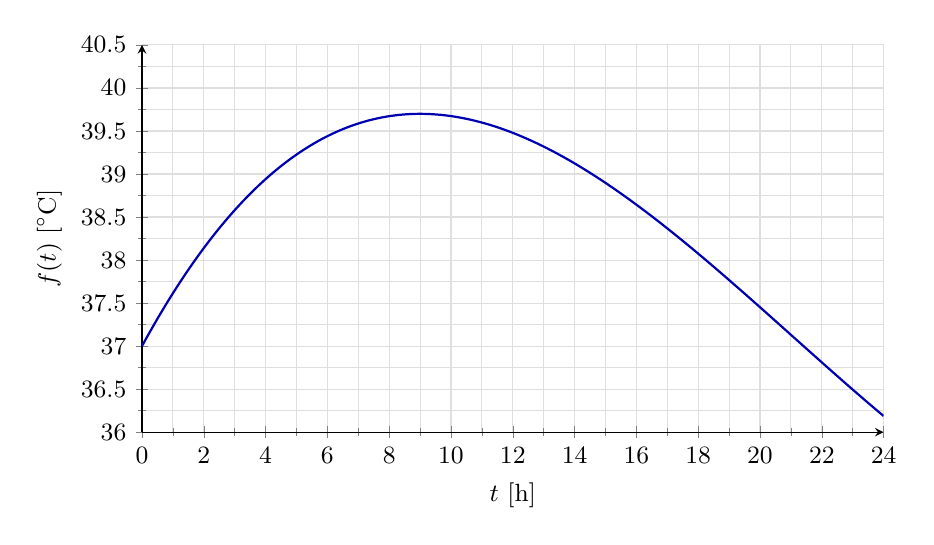
\begin{tikzpicture}
\begin{axis}[
  width=11cm, height=6.5cm,
  xmin=0, xmax=24, ymin=36, ymax=40.5,
  xlabel={$t$ [h]}, ylabel={$f(t)$ [$^\circ$C]},
  axis lines=left, grid=both, grid style={gray!25},
  minor tick num=1,
  xtick={0,2,...,24}, ytick={36,36.5,...,40.5},
  tick label style={font=\small}, label style={font=\small},
  samples=200, domain=0:24,
]
\addplot[thick, blue!70!black] {0.00074*x^3-0.04667*x^2+0.66*x+37};
\end{axis}
\end{tikzpicture}
\end{center}

\subexercise{
Bestimmen Sie mit dem Graphen die höchste Fiebertemperatur.
\solve{
Der Graph erreicht sein Maximum bei $t\approx9$ mit einer Temperatur von etwa $39{,}7\,^\circ\mathrm C$.\pp[2]
}
}
\vskip8pt
\subexercise{
Ab $38\,^\circ\mathrm C$ spricht man von Fieber. Markieren Sie im Graphen den Zeitraum, in dem Fieber vorliegt.
\solve{
Der Graph verläuft oberhalb von $38\,^\circ\mathrm C$ etwa im Bereich $1{,}7\le t\le18{,}3$ -- dieser Zeitraum ist im Graphen zu markieren.\pp[2]
}
}
\vskip8pt
\subexercise{
Bestimmen Sie näherungsweise mit dem Graphen den Zeitpunkt, ab dem die Temperatur wieder unter $37\,^\circ\mathrm C$ liegt.
\solve{
Der Graph unterschreitet $37\,^\circ\mathrm C$ bei etwa $t\approx21{,}4$, also nach ungefähr $21$ Stunden und $24$ Minuten.\pp[2]
}
}
\vskip8pt
\subexercise{
Erklären Sie die Bedeutung der Zahl $37$ in der Funktionsgleichung.
\solve{
$f(0)=37$: Zu Beginn der Beobachtung ($t=0$) beträgt die Temperatur $37\,^\circ\mathrm C$, also die normale Körpertemperatur.\pp[2]
}
}
\vskip8pt
\subexercise{
Bestimmen Sie den Grenzwert von $f(t)$ für $t\to\infty$ und erklären Sie damit, warum man $f$ nur für $0\le t\le24$ betrachten sollte.
\solve{
\[
\lim_{t\to\infty}f(t)=\infty
\]
\pp Eine Körpertemperatur kann nicht unbegrenzt weiter ansteigen -- außerhalb von $0\le t\le24$ beschreibt der Funktionsterm keinen sinnvollen Temperaturverlauf mehr, das Modell verliert dort seine Bedeutung.\pp[2]
}
}
\vskip8pt
\subexercise{
Zwischen Stunde $16$ und Stunde $22$ nimmt die Temperatur näherungsweise linear ab.

(i) Berechnen Sie die Temperatur zu beiden Zeitpunkten.

(ii) Bestimmen Sie eine lineare Funktion $g(t)=mt+b$, die den Temperaturverlauf in diesem Zeitraum beschreibt.
\solve{
(i)
\[
f(16)\approx38{,}6\,^\circ\mathrm C,\qquad f(22)\approx36{,}8\,^\circ\mathrm C
\]
\pp[2]

(ii)
\[
m=\frac{36{,}8-38{,}6}{22-16}=\frac{-1{,}8}{6}=-0{,}3
\]
Einsetzen: $38{,}6=-0{,}3\cdot16+b\Rightarrow b=43{,}4$.
\[
g(t)=-0{,}3t+43{,}4
\]
\pp[3]
}
}
}

\newpage
\exercise*[Aufgabe 4]{
Für ein Skatepark-Element (eine sogenannte \emph{Wave}) wird die Auslenkung der Fahrbahn gegenüber einer Bezugslinie für $-9\le x\le9$ (in Metern) durch die Funktion
\[
h(x)=-0{,}01x^3+0{,}81x
\]
modelliert. Dabei ist $x$ die waagerechte Entfernung von der Mitte der Anlage in Metern und $h(x)$ die Auslenkung in Metern.

\subexercise{
Berechnen Sie $h(3)$ und deuten Sie das Ergebnis im Sachzusammenhang.
\solve{
\[
h(3)=-0{,}01\cdot27+0{,}81\cdot3=-0{,}27+2{,}43=2{,}16
\]
\pp Bei $3\,\mathrm m$ Entfernung von der Mitte liegt die Fahrbahn $2{,}16\,\mathrm m$ oberhalb der Bezugslinie.\pp
}
}

\subexercise{
Bestimmen Sie rechnerisch die Nullstellen von $h$.
\solve{
\[
-0{,}01x^3+0{,}81x=0
\]
\[
x(-0{,}01x^2+0{,}81)=0
\]
\pp[2] $x=0$ oder $-0{,}01x^2+0{,}81=0 \Rightarrow x^2=81 \Rightarrow x=9$ oder $x=-9$.
\[
x_1=-9,\qquad x_2=0,\qquad x_3=9
\]
\pp[2]
}
}

\subexercise{
Weisen Sie rechnerisch nach, dass der Graph von $h$ punktsymmetrisch zum Ursprung ist, und deuten Sie diese Eigenschaft im Sachzusammenhang.
\solve{
\[
h(-x)=-0{,}01(-x)^3+0{,}81(-x)=0{,}01x^3-0{,}81x=-h(x)
\]
Also ist $h$ punktsymmetrisch zum Ursprung.\pp[2] Im Sachzusammenhang bedeutet das: Die Fahrbahn verläuft auf beiden Seiten der Mitte spiegelbildlich (mit umgekehrtem Vorzeichen der Auslenkung).\pp
}
}

\subexercise{
Erläutern Sie, warum das Modell sinnvollerweise nur für $-9\le x\le9$ verwendet wird.
\solve{
Bei $x=-9$ und $x=9$ nimmt $h$ den Wert $0$ an (siehe Nullstellen) -- dort trifft die Fahrbahn wieder auf die Bezugslinie, das Bauwerk endet an diesen Stellen. Außerhalb dieses Bereichs beschreibt der Funktionsterm keine reale Fahrbahn mehr, das Modell verliert dort seine Bedeutung.\pp[2]
}
}
\vskip8pt
\subexercise{
Die Fahrbahn beginnt und endet jeweils an einem \emph{Einstiegspunkt}. Bestimmen Sie die Entfernung zwischen den beiden Einstiegspunkten der Wave.
\solve{
Die Einstiegspunkte liegen bei $x=-9$ und $x=9$ (siehe Nullstellen). Die Entfernung beträgt
\[
9-(-9)=18\,\mathrm m.
\]
\pp
}
}
\vskip8pt
\subexercise{
Berechnen Sie die Höhe der Fahrbahn an den beiden Einstiegspunkten.
\solve{
\[
h(-9)=-0{,}01\cdot(-729)+0{,}81\cdot(-9)=7{,}29-7{,}29=0
\]
\[
h(9)=-0{,}01\cdot729+0{,}81\cdot9=-7{,}29+7{,}29=0
\]
An beiden Einstiegspunkten liegt die Fahrbahn auf Höhe der Bezugslinie ($0\,\mathrm m$).\pp[2]
}
}
}

\vskip20pt
\textbf{Zugelassene Hilfsmittel für Prüfungsteil B:}
\begin{itemize}
\item CAS-Taschenrechner
\item Formelsammlung
\item Wörterbuch zur deutschen Rechtschreibung
\end{itemize}

\end{exam}
\end{document}